\documentclass[a4paper]{article}
\usepackage[14pt]{extsizes} % для того чтобы задать нестандартный 14-ый размер шрифта
\usepackage[utf8]{inputenc}
\usepackage[english, russian]{babel}
\usepackage{setspace,amsmath}
\usepackage {graphicx}
\usepackage[left=12mm, top=15mm, right=12mm, bottom=15mm, nohead, footskip=10mm]{geometry} % настройки полей документа
\usepackage{tabularx}
\begin{document}
	{\Large Лабораторная работа 3.4.1}
	\hfill \break
	\hfill \break
	\hfill \break
	{\LARGE Диа- и парамагнетики 
	}
	\hfill \break
	\hfill \break
	{\normalsize \textbf{Цель работы:}  змерение магнитной восприимчивости диа- и парамагнитных образцов.}
	
	\hfill \break
	\hfill \break
	{\normalsize \textbf{В работе используются:} электромагнит, аналитические весы, милливеберметр, регулируемый источник постоянного тока, образцы.
	}
	\hfill \break
	\hfill \break
	\section{Теоретические сведения}
Магнитная восприимчивость тел может быть определена методом измерения сил, которые действуют на тела в магнитном поле. Существуют два классических метода таких измерений: метод Фарадея и метод Гюи. В методе Фарадея исследуемые образцы, имеющие форму маленьких шариков, помещаются в область сильно неоднородного магнитного поля и измеряется сила, действующая на образец. При этом для расчёта магнитной восприимчивости необходимо знать величину градиента магнитного поля в месте расположения образца. В методе Гюи используется тонкий и длинный стержень, один из концов которого помещают в зазор электромагнита (обычно в область однородного поля), а другой конец -- вне зазора, где величиной магнитного поля можно пренебречь. Закон изменения поля -- от максимального до нулевого -- в этом случае несуществен.

Найдём выражение для магнитной силы, действующей на такой образец (рис. \ref{pic:2}). Пусть площадь образца равна $ s $, его магнитная проницаемость -- $ \mu $, а поле в зазоре равно $ B $.

\begin{figure}[h!]
	\centering
	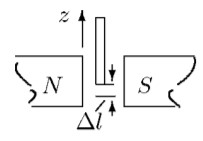
\includegraphics[width=5cm]{/home/kun02/llab/Screenshot_2.jpg}
	\caption{Расположение образца в зазоре электромагнита}
	\label{pic:2}
\end{figure}

Воспользуемся для расчёта энергетическими соображениями. Магнитная сила может быть вычислена как производная от магнитной энергии по перемещению. Из теории известно, что эту производную следует брать со знаком минус, когда образец находится в поле постоянного магнита, или со знаком плюс, как в нашем случае, когда поле в зазоре создаётся электромагнитом, ток $ I $ в обмотках которого поддерживается постоянным.

При смещении образца на расстояние $ \Delta l $ вниз магнитная сила, действующая на него, равна

\begin{equation}\label{1}
	F = \left(\frac{\Delta W_m}{\Delta l}\right)_I,
\end{equation}
где $ \Delta W_m $ -- изменение магнитной энергии системы при постоянном токе
в обмотке электромагнита и, следовательно, при постоянной величине
магнитного поля в зазоре.

Магнитная энергия рассчитывается по формуле

\begin{equation}\label{2}
	W_m=\frac{1}{2}\int HBd\,V = \frac{1}{2\mu_0}\int\frac{B^2}{\mu}d\,V,
\end{equation}
где интеграл распространён на всё пространство. При смещении образца магнитная энергия меняется только в области зазора (в объёме площади $ s $ и высоты $ \Delta l $), а около верхнего конца стержня остаётся неизменной, поскольку магнитного поля там практически нет. Принимая поле внутри стержня равным измеренному нами полю в зазоре $ B $, получим

\begin{equation}\label{3}
	\Delta W_m=\frac{1}{2\mu_0}\frac{B^2}{\mu}s\Delta l - \frac{1}{2\mu_0}B^2 s\Delta l = -\frac{\chi}{2\mu_0\mu}B^2s\Delta l.
\end{equation}

Следовательно, на образец действует сила

\begin{equation}\label{4}
	F = -\frac{\chi}{2\mu_0\mu}B^2S.
\end{equation}

Знак силы, действующей на образец, зависит от знака $ \chi $: образцы из парамагнитных материалов $( \chi  > 0)$ втягиваются в зазор электромагнита, а диамагнитные образцы $ (\chi < 0) $ выталкиваются из него.

Пренебрегая отличием $ \mu $ от единицы, получаем окончательно расчётную формулу в виде

\begin{equation}\label{5}
	F = -\frac{\chi B^2S}{2\mu_0}.
\end{equation}

Измерив силу, действующую на образец в магнитном поле $ B $, можно рассчитать магнитную восприимчивость образца.

\section{Экспериментальная установка}

\begin{figure}[h!]
	\centering
	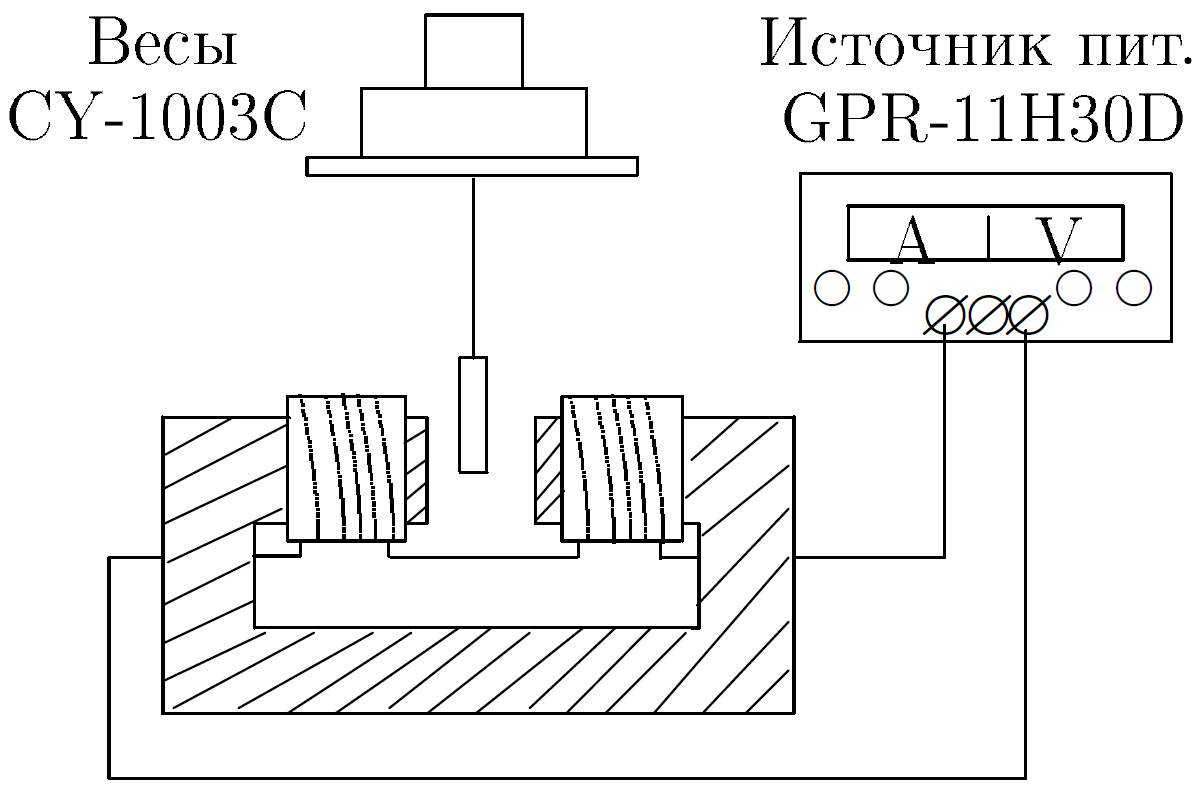
\includegraphics[width=7.6cm]{/home/kun02/llab/Screenshot_1.png}
	\caption{Схема экспериментальной установки.}
	\label{pic:1}
\end{figure}


Магнитное поле с максимальной индукцией $ \simeq 1 $ Т создаётся в зазоре электромагнита, питаемого постоянным током. Диаметр полюсов существенно превосходит ширину зазора, поэтому поле в средней части зазора достаточно однородно. Величина тока, проходящего через обмотки электромагнита, задаётся регулируемым источником питания GPR и измеряется амперметром $ А $, встроенным в источник питания. Градуировка электромагнита (связь между индукцией магнитного поля $ B $ в зазоре электромагнита и силой тока $ I $ в его обмотках) производится при помощи милливеберметра.


При измерениях образцы поочерёдно подвешиваются к весам так, что один конец образца оказывается в зазоре электромагнита, а другой -- вне зазора, где индукцией магнитного поля можно пренебречь. При помощи весов определяется перегрузка $ \Delta P = F $ -- сила, действующая на образец со стороны магнитного поля.


Силы, действующие на диа- и парамагнитные образцы, очень малы. Небольшие примеси ферромагнетиков (сотые доли процента железа или никеля) способны кардинально изменить результат опыта, поэтому образцы были специально отобраны.

\section{Ход работы}
\begin{enumerate}
	\item Построим градуировочную криваую для электромагнита и расчитаем поле В
	\hfill\break $SN = 72 (\text{см})^2 \qquad r= 5 \text{см}$
	
	\begin{center}
	\begin{tabular}{|c|c|c|c|c|c|c|c|c|} \hline
	
	$N$ &1&2&3&4&5&6&7&8 \\ \hline
	$I$, A & 0,28 &0,65&1,21&1,6&1,91&2,3&2,72& 3,01 \\ \hline
	$d\Phi$, мВб &0,6&1,3&2,6&3,6&4,2&5,1&5,6&6,1  \\ \hline
	
	\end{tabular}
\end{center}
\begin{figure}[h!]
	\centering
	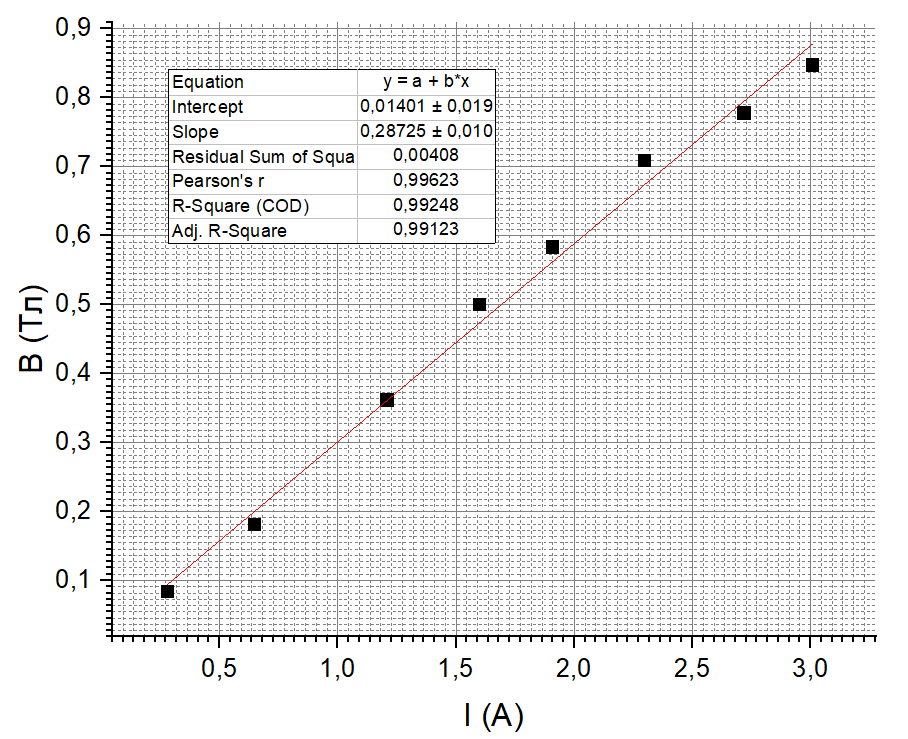
\includegraphics[width=18cm]{/home/kun02/llab/3.4.1-1.png}
	\caption{Градуировочная кривая B(I)}
	\label{pic:1}
\end{figure}
\par Из графика следует: $k = 0,287 \pm 0,01 \text{Тл/A}$
	\item $d = 1  \text{см} \quad m_{cu} = 83, 169 \text{г} \qquad m_{Al} = 25 255 \text{мг} \qquad m_{W} = 151 281 \text{мг}  \qquad m_{C} = 12 899 \text{мг}$
		\begin{center}
		\begin{tabular}{|c|c|c|c|c|c|c|c|c|} \hline
			
			$N$ &1&2&3&4&5&6&7&8 \\ \hline
			$I$, A & 0,28 &0,65&1,21&1,6&1,91&2,3&2,72& 3,01 \\ \hline
			$dP_{cu} \pm 15$, мг &5&6&8&11&13&17&22&24 \\ \hline
			$dP_{Al} \pm 15$, мг &1&-2&-9&-17&-23&-31&-42&-50 \\ \hline
			$dP_{W} \pm 15$, мг &2&9&32&63&76&105&139&162\\ \hline
			$dP_{C} \pm 15$, мг &8&21&42&48&49&40&28&17\\ \hline
		\end{tabular}
	\end{center}
	\begin{figure}[h!]
		\centering
		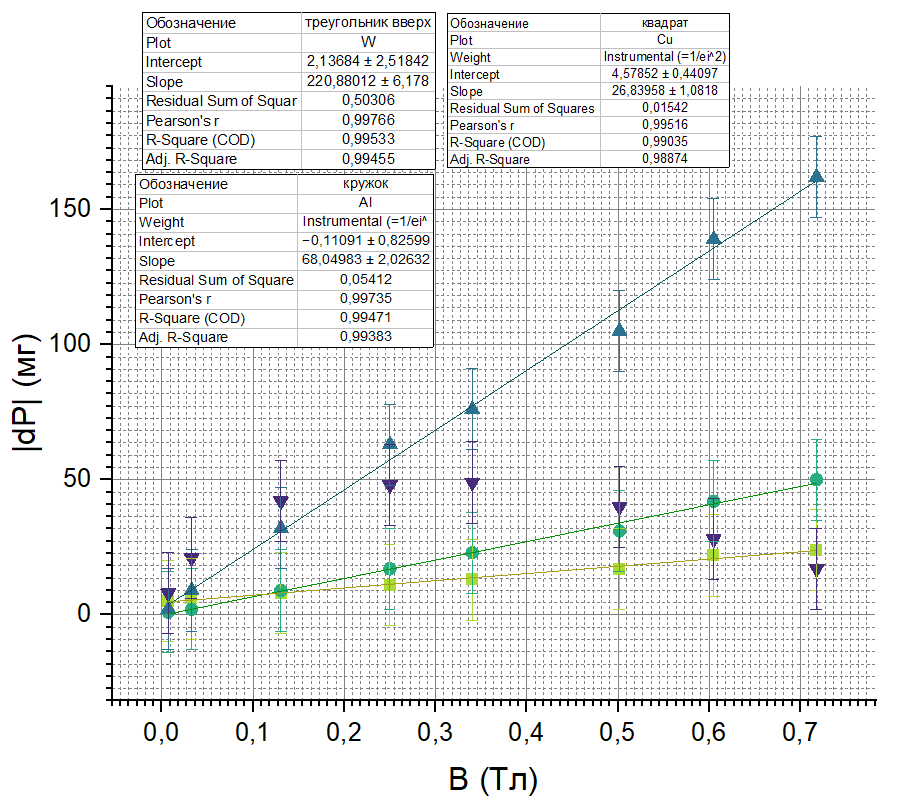
\includegraphics[width=18cm]{/home/kun02/llab/3.4.1-2.png}
		\caption{|dP|($B^2$)}
		\label{pic:1}
	\end{figure}
\par Расчитаем на форлуме (5) магнитную восприимчивость $\chi$, для графита посчитать не сможем, поскольку график аппроксимировать прямой нельзя, где $S = \pi d^2/4$
\begin{center}
	\begin{tabular}{|c|c|c|c|} \hline
		материал&Cu&Al&W \\ \hline
		$\chi \cdot 10^{-6}$, $\text{$\text{м}^3$/кг} $&-(8,6$ \pm 6,4$)& 21,7 $\pm 6,4$ & 70,7 $\pm 6,7$ \\ \hline
		$\varepsilon$, $\%$ & 75 & 30 & 9 \\ \hline
		
	\end{tabular}
\end{center}
\section{Вывод}
Эксперементально были получены магнитные восприимчивость Cu, Al, W. С учетом погрешностей данные совпадают с табличными. Основной погрешностью измерение является погрешность весов, значительно в некоторых случиях превышающую измеряемою величину изменения силы. Получается медь диамагнетик $\chi $ < 0, аллюминий и вольфрам парамагненетики. Несмотря на то, что графит должен демонстрировать диамагнетизм, в нашем опыте он обладает парамагнитными свойствами. Это могло произойти из-за того, что исследуемый образец имел недостаточную длину и не мог полностью оказаться между двух обкладок электромагнита. Вследствие этого могли возникнуть некоторые неточности в ходе измерения истинного поведения образца в магнитном поле. Кроме того, о неточности опытов также говорит нарушение линейности графика зависимости $ |\Delta P|(B^2) $. Из-за со-держания определенного рода дефектов графит способен к самопроизвольному намагничиванию, что мы и наблюдали в данном эксперименте.
\end{enumerate}	
\end{document}